\chapter{定量脑电谱质量筛选的谱同构准则}
\section{研究背景}
前面三章主要研究定量脑电中的参考选择问题。与参考类似关系到脑电数据质量还有如何对大样本数据进行质量筛选。发展集成脑电数据处理流水线平台的挑战在于最初预处理,该阶段需要去除脑电伪差还要尽可能保留与大脑活动有关的脑电信号。已有脑电预处理流水线平台均依赖质量指标,根据指标可对单通道信号或一段信号去除伪差或矫正。脑电信号要经过滤波和基于独立成分分析去除伪差成分。评估脑电预处理流程软件结果时发现多通道$\log$谱相互平行的问题,如图\ref{5:issue}A所示所有电极谱相互平行。本章提出能评估脑电频谱电极间相互平行程度或者交叉谱同构程度的PaLOS准则并在不同数据库和预处理步骤中得到验证。

神经电生理大数据的出现需要相应的批量自动化处理程序\citing{bigdely-shamlo_prep_2015}如自动化伪差去除\citing{jas2017autoreject}、自动正演模型求解\citing{huang2019realistic,vorwerk2018fieldtrip}、自动溯源分析\citing{niso2019brainstorm,weinstein2001biopse}及自动统计分析。不可或缺的是对自动化程序进行质量控制代替专家监督自动化处理程序\citing{jas2018reproducible}。利用脑电等电生理技术的高时间分辨率和频谱分析技术,人们希望刻画神经源连接的空间模式作为脑认知功能和精神紊乱的潜在生物标记物\citing{friston2011functional,jirsa2007handbook,mars2018connectivity,schoffelen2009source}。自动化数据分析的第一步是筛选脑电脑磁数据、去除伪差等。然后更通常的是对时域波形进行谱估计输出交叉谱,
交叉谱代表大脑活动的全部动力学信息\citing{nolte2019mathematical,siegel2012spectral}。最后溯源方法转换头表空间的交叉谱到神经源空间\citing{bosch20013d}。尽管已存在一些自动化脑电磁数据预处理程序如Automagic\citing{pedroni2019automagic}、Autoreject\citing{jas2017autoreject}、PREP\citing{bigdely-shamlo_prep_2015}、HAPPE\citing{gabard2018harvard}、APP\citing{da2018automatic}和加拿大布鲁克大学心理学院开发的lossless(https://github.com/BUCANL/BIDS-Lossless-EEG),尚没有一个能检查伪差去除后的频域失真。实际中尽管难知道脑电磁数据无噪声信号的基标准,但应用越多越复杂的伪差去除程序可能去除与脑活动相关的信号。用强力算法进行伪差去除后得到的好看脑电波形可能离大脑活动的内在动力学相差较远或改变了大脑源活动的连接空间模式。
\begin{figure}[!h]
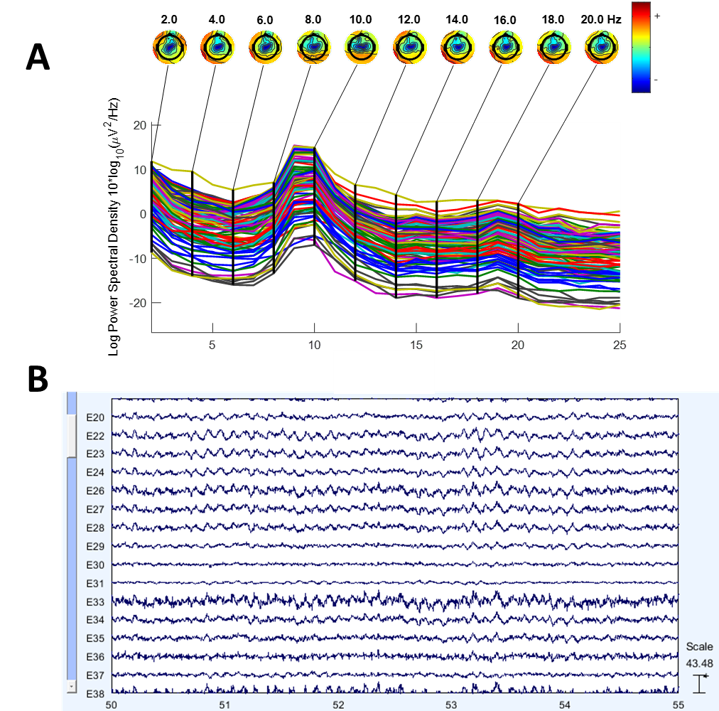
\includegraphics[width=15cm]{pic/palos/issue.png}
\caption{多通道功率谱同构问题示例。 A.被试数据经Automagic\citing{pedroni2019automagic}预处理后的功率谱, 不同颜色的曲线代表不同电极的功率谱,可看出功率谱曲线高度平行不同频率下的谱地形图分布很相似;B.经Automagic预处理后被认为是干净脑电数据的波形。}
\label{5:issue}
\end{figure}

电生理神经成像将无创记录到的脑电数据视为大脑活动信号,敏感的电极传感器容易使微弱脑电信号淹没在各种各样的噪声中,采集的数据波形通常不很好看。无论脑电数据经过怎样的预处理,进一步分析动力学或源活动的必要步骤是对头表上估计到的频谱进行质量分析。我们发现$\log$转换后的频谱在所有电极间相互平行即存在谱同构(Parallel LOg Spectra,PaLOS)问题。如图\ref{5:issue}所示,较短频率间隔上的谱地形图呈现稳定相似的空间模式可能表明神经源偶极子的振荡配置基本稳定,与大脑具有高度依赖于频率振荡的动力学信息这一认识相背离\citing{cabral2017functional,
deco2011emerging}。也有研究认为大脑连接更可能依赖于频率呈现不同模式而非静态固定的\citing{chang2010time,foster2015intrinsic,hacker2017frequency,thompson2015frequency}。这种头表谱地形图在不同频率间非常相似预示着神经源空间在所有频率存在相近位置上相似的偶极子活动,脑电的实际源可能因为去除过多伪差而难以识别,违背了不同频率下不同神经元共振模式的事实\citing{hacker2017frequency}。

本章提出用各个频率下共同正交基的第一个主成分\citing{trendafilov2010stepwise}在交叉谱数据中所有频率上占的比例作为判定伪差去除后的脑电脑磁数据是否具有谱同构问题的PaLOS准则。直观推理,如果多通道功率谱在所有频率上电极间相互平行,所有通道的谱曲线就是一条共同的主要谱曲线加减不同尺度平移后的结果。多通道功率谱相互平行这个单变量问题可推广到多变量交叉谱的情况,所有频率下交叉谱由共同交叉谱空间模式的尺度变换合成且其中一个在解释全局方差中绝对占优。为验证PaLOS准则,一方面在不同样本量不同预处理情况的数据库上比较,还考虑一些人为可能引入PaLOS问题的处理步骤如转换参考\citing{hu_how_2018}、坏道选择、滤波、使用独立成分分析进行伪差去除,插值修复坏道、眼电回归等。 

\section{研究方法}
\subsection{谱同构模型}
图\ref{5:issue}A表示多通道功率谱同构的现象,多通道功率谱在$\log_{10}$上相互平行,可表示为
\begin{equation}\label{eq5.1}
\log_{10}\mathbf{p}^\omega=\mathbf{c}+\log_{10}\bar{p}^\omega
\end{equation}
这里$\mathbf{p}^\omega$指频率点$\omega$下所有电极的功率谱,$\bar{p}$是单频率点下所有电极功率谱平均值,$\mathbf{c}$是一
列由各个电极上的偏差常数组成的向量。

$\log_{10}$上相互平行的功率谱转换到自然尺度上就是单个频率点上成比例的功率谱,关于电极$e(e=1,...,N_e)$可以表示为
\begin{equation}\label{eq5.2}
\mathbf{p}^\omega=10^\mathbf{c}\bar{p}^\omega,\quad{p}_e^\omega=10^{c_e}\bar{p}^\omega
\end{equation}

因为谱的方差意义,考虑对单频率下大小为所有电极$\times$所有数据段的傅里叶系数矩阵进行主成分分析,记负载(loadings)矩阵为$\mathbf{L}^\omega$,记白化(whitening)矩阵为$\mathbf{\Gamma}^T=[\mathbf{\gamma}_1,...,\mathbf{\gamma}_{N_e}]$,逐个电极上的功率谱可记为
\begin{equation}\label{eq5.3}
\mathbf{L}^\omega=\mathbf{\Gamma}\mathbf{D^{1/2}}^\omega,\quad{p}_e^\omega=\mathbf{\gamma}_e^T\mathbf{D}^\omega\mathbf{\gamma}_e
\end{equation}
这里$\mathbf{\Gamma}$是正交阵,服从$\mathbf{\Gamma}\mathbf{\Gamma}^T=\mathbf{I}_{N_e}$,$\mathbf{D}$是由特征值平方组成的对角阵。不妨通过主成分分析把多通道电极功率谱在自然尺度上成比例
转换为傅里叶系数负载矩阵在第一个电极上对应的特征值占优。

多通道功率谱是多通道电极间交叉谱的对角元,记交叉谱为$\mathbf{S}^\omega$,对频率点$\omega(\omega=1,...,N_\omega)$下的大小为所有电极
$\times$所有数据段的傅里叶系数矩阵都进行主成分分析。因为多通道功率谱同构是所有电极功率谱关于频率的曲线相互平行,可推断不同频率下多通道电极间的交叉谱矩阵具有相似的主成分空间\citing{boik1988common,krzanowski1984principal},对所有频率下交叉谱矩阵采用具有共同正交基的主成分分析\citing{trendafilov2010stepwise}得到
\begin{equation}\label{eq5.4}
\mathbf{S}^\omega=\mathbf{\Gamma}\mathbf{D}^\omega\mathbf{\Gamma}^T
\end{equation}
这里$\mathbf{\Gamma}$不随频率变化,$\mathbf{D}^\omega$作为由交叉谱矩阵的特征值平方组成的对角矩阵随频率变化。\eqref{eq5.4}是从单变
量的多通道电极功率谱平行到多变量的多通道电极交叉谱同构的推广。图\ref{5:tensor}是幅度平方归一化的多通道电极交叉谱(幅度平方相干)在所有频率下的示意图,图\ref{5:issue}A中所有电极的功率谱在$\log_{10}$尺度上关于频率的谱曲线平行可看作图\ref{5:tensor}中每个频率点下所有电极交叉谱矩阵的对角线值随频率变化的曲线相互之间成比例。
\begin{figure}[!h]
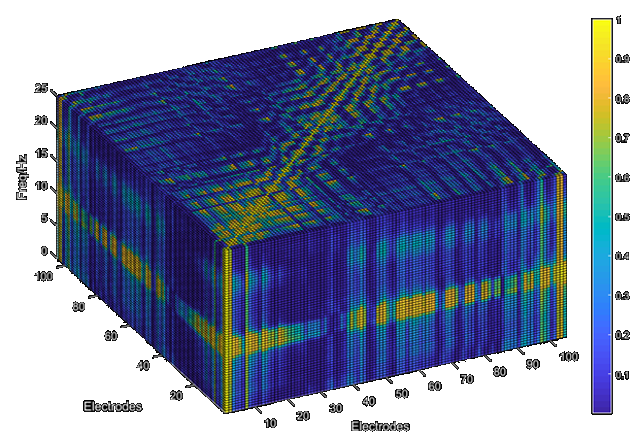
\includegraphics[width=11cm]{pic/palos/spectratensor.png}
\caption{多频率点下幅度平方归一化的交叉谱(幅度平方相干)矩阵示意图。}
\label{5:tensor}
\end{figure}

\subsection{谱同构指数}
谱曲线的平行程度或交叉谱矩阵的同构程度可由交叉谱矩阵最主要占优的成分比例来说明。谱同构指数(PaLOS index)用公式表示为
\begin{equation}\label{eq5.5}
r=\frac{\sum_{\omega=1}^{N_\omega}\mathbf{D}^\omega(1,1)}{\sum_{\omega=1}^{N_\omega}\Tr(\mathbf{S}_\omega)}
\end{equation}
主成分分析的正交线性转换过程中每一步是在最大化关于转换向量的瑞利熵(Rayleigh quotient),最大化的结果得到特征值$\mathbf{D}(e,e)$\citing{Jolliffe2002}。

对任意的$\mathbf{S}^\omega$进行主成分分析都满足$\Tr(\mathbf{S}_\omega)=\sum_{e=1}^{N_e}\mathbf{D}(e,e)$,因此0<r$\leq$1。我们称
$r$为谱的同构异质性指数,$r$越大表示谱具有很强的同构性则数据质量可能越差,$r$越小表示谱具有很强的异质性则数据质量可能越好。

\subsection{影响因素}
为验证谱同构准则表示数据预处理程度特别是伪迹去除、脑电信号丢失的有效性,还需要考虑一些可能会影响数据同构异质性的因素。
\subsubsection{参考问题}
参考问题是本论文的主要研究内容之一。第四章发现参考变换矩阵$\rank{(\mathbf{T})}=N_e-1$具有满秩减一属性,因此$N_e$通道脑电数据的秩至多为$N_e-1$。用$\mathbf{T}$表示参考变换矩阵,交叉谱随参考变换的过程表示为
\begin{equation}\label{eq5.6}
\mathbf{v}_r=\mathbf{T\phi},\quad\mathbf{S}_r=\mathbf{T}\Sigma_\mathbf{\phi\phi}\mathbf{T}^T
\end{equation}
这里清楚地表示交叉谱矩阵随不同参考而变化。本章比较的几种参考是Cz、传统平均参考、鲁棒平均参考和零参考。鲁棒平均参考是通过迭代鲁棒地估计平均参考信号,以不受噪声等离群值的影响\citing{lepage2014statistically}。尽管交叉谱矩阵受参考影响,利用单极参考的无记忆性\citing{hu_statistics_2019}容易重参考交叉谱矩阵为另一种参考,过程如下
\begin{equation}\label{eq5.7}
\mathbf{S}_{r_2}=\mathbf{T}_{r_2}\mathbf{S}_{r_1}\mathbf{T}_{r_2}^T
\end{equation}
由此可得理论上重参考过程可直接在交叉谱之间进行,不需要回到原始脑电数据进行参考变换再进行预处理。

\subsubsection{预处理分析}
预处理分析一般包括软件分析和专家挑选。多种预处理分析软件大多基于独立成分分析,区别在于预处理步骤不同,如Prep\citing{bigdely-shamlo_prep_2015}、MARA\citing{winkler2011automatic}、FASTER\citing{nolan2010faster}、ADJUST\citing{mognon2011adjust}、SASICA\citing{chaumon2015practical}和Automagic\citing{pedroni2019automagic}等。其中Automagic是一种包含预处理步骤最多,集成现成预处理工具包的功能如Prep中坏道挑选和MARA中伪差成分去除并具有质量控制功能的一体化预处理分析软件。Automagic的预处理步骤分为原始数据(Raw/Orig)、坏道挑选(Prep)、滤波(Filt)、眼电回归(Reg)、伪差成分去除(MARA)、插值(Itpl)、质量评价(Asse)等阶段。这些预处理软件旨在通过一系列步骤去除尽可能多的伪差信号,从幅度、方差、坏道比例、插值比例等分析脑电时域信息,直到处理最终脑电信号具有如图\ref{5:issue}B所示好看的波形。与此不同,专家挑选是神经电生理专家根据经验和知识通过视觉手动筛选出波形较为平稳接近线性变换适合定量分析的数据段,去除明显漂移、心电、肌电等伪差以及明显非线性非稳态波动的数据段。

软件分析与专家挑选各有利弊,软件分析更加客观但无法判定独立成分波形的生理意义,可能为刻意追求好看波形去除与脑活动有关的信号,可能通过回归、插值等增大数据共线性,专家检测依赖于专家自身的经验和知识并可能受到研究目的等动机影响但一般不易丢弃与脑活动有关的成分。
\begin{figure}[!h]
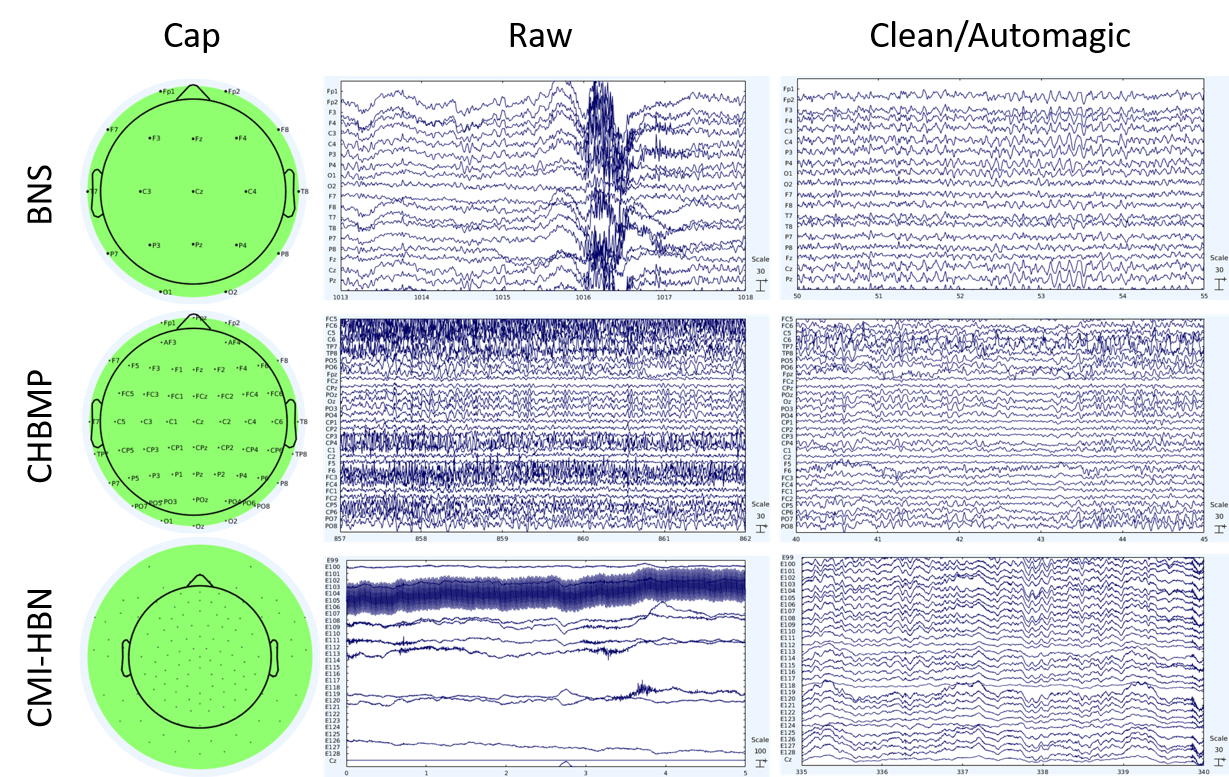
\includegraphics[width=15cm]{pic/palos/data.png}
\caption{谱同构准则测试数据库样本示例。BNS:巴巴多斯营养不良研究脑电数据库,CHBMP:古巴人脑影像数据库,CMI-HBN:美国儿童脑智研究院人脑网络数据库。BNS和CHBMP的Clean数据是经专家挑选的稳态脑电数据,CMI-HBN Automagic是原始数据经Automagic软件预处理后的数据。}
\label{5:database}
\end{figure}

\section{数据}
这里希望在样本量不同且电极配置不同的数据集中验证谱同构准则。我们从如图\ref{5:database}中三个不同的数据库收集脑电数据:1. 美国纽约儿
童脑智研究院-人脑网络(CMI-HBN)数据库\citing{alexander2017open},采用129通道按照GSN系统分布的EGI电极帽,采集频率为500Hz,1224例健康被试的静息态脑电数据,每一例数据包括原始数据和使用Automagic预处理后的数据;2.古巴人脑影像(CHBMP)数据库\citing{hernandez-gonzalez_multimodal_2011},采用58通道按照10-10电极放置系统分布的电极帽,采集频率为200Hz,250例健康被试的静息态脑电数据,每一例数据包含原始数据和专家挑选的稳态脑电数据;3. 巴巴多斯儿童大脑发育与营养不良关系的研究\citing{BringasVega2019}(BNS)项目数据库,使用19通道按照10-20电极放置系统分布的电极帽,采集频率为200Hz,采集的51例健康被试静息态脑电数据,每一例数据包含原始数据和专家挑选的稳态脑电数据。CMI-HBN数据被试是儿童和青少年,CHBMP数据被试覆盖整个生命周期,BNS数据被试是45-51岁左右的成年人。三个数据库的原始脑电数据采集条件相当,都是静息态闭眼脑电。

从图\ref{5:database}可看出,CMI-HBN的原始数据质量最差,含有大量电极漂移和高频噪声等,经过Automagic预处理后数据波形看上去较为平稳;CHBMP和BNS的原始数据在某些电极上或数据段内具有明显伪差,经专家视觉挑选稳态数据段后数据非常平稳。

\section{结果与讨论}
\subsection{谱同构指数在数据库上的验证}
这里分别应用谱同构准则到以上三个数据库共1525例健康被试的脑电数据。CMI-HBN数据库中1224例脑电数据一方面来自儿童和青少年,其次使用了高密度GSN129型电极帽,采集到较多眼电,波动漂移、高幅、高频数据非常明显且包含有很多难以描述类型的伪差。CHBMP中250例来自整个生命周期的数据,采用较为稀疏的58通道,有少量眼电和部分数据段上波动伪差、某些电极高阻抗产生的伪差等。BNS中51例数据来自中年人,采用最稀疏的19通道,基本没有采集到眼电,数据段偶尔呈现因被试头动产生的伪差。对每一例数据首先按照2.56s的窗长分段再使用multitaper方法\citing{thomson1982spectrum}计算交叉谱,平滑参数时半带宽积为3.5,最大频率为25Hz。 CMI原始数据和Automagic都是按照Cz作为参考来计算,因此这里对CHBMP和BNS的数据都采用Cz参考。尽管参考对谱计算有一定影响,但单极参考间的相互变换不会改变脑电数据质量太多,因此在数据库上计算PaLOS准则并没有比较平均参考和零参考。PaLOS准则受参考因素的影响见下一节。
\begin{figure}[!h]
	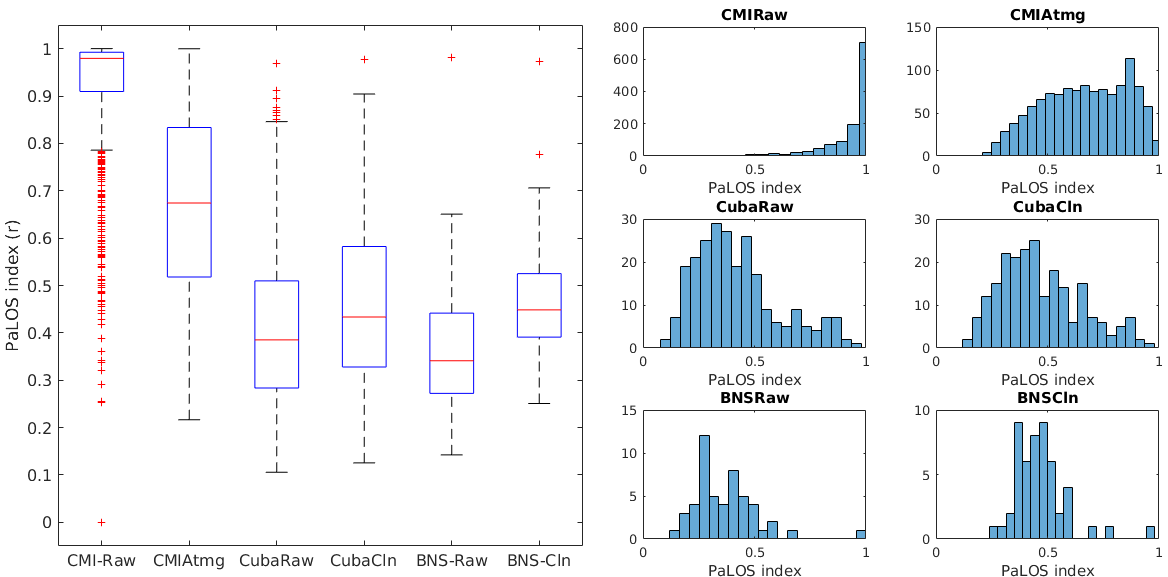
\includegraphics[width=15cm]{pic/palos/comparison.png}
	\caption{谱同构指数数据间对比。CMI-Raw:CMI-HBN原始数据,CMIAtmg:使用Automagic预处理后的CMI-HBN数据,CubaRaw:CHBMP原始数据,CubaCln:CHBMP经专家挑选的稳态数据段,BNSRaw:BNS数据库中原始数据,BNSCln:BNS数据库中经专家挑选的稳态数据段。}
	\label{5:comp}
\end{figure}

从图\ref{5:comp}中柱状图和直方图可看出CMI数据库上的谱同构准则(PaLOS index)中值从原始数据时的0.98减小到使用Automagic预处理后的0.66,而Cuba的CHBMP数据库从原始数据的0.38增加到专家挑选后稳态数据段的0.42,巴巴多斯BNS数据库从原始数据的0.34增加到专家挑选后稳态数据段的0.43。该结果与预料的一致,因为CMI原始数据含有大量冗余噪声脑电信号几乎被完全淹没,交叉谱由于噪声高度同构,谱同构指数主要聚集在接近1的位置,使用Automagic进行预处理去除坏道和明显伪差后的数据质量因为被试个体差异有所不同,交叉谱反映出更加体现脑电在大样本被试上的个体差异,谱同构指数下降到中值为0.66但呈现更加离散的分布;古巴CHBMP数据库和巴巴多斯BNS数据库因为采用相同型号的脑电采集设备(Neuronic)且主试对数据采集质量控制较好,两个数据库中原始数据仅具有较少眼电和时间段较短的明显伪差,另外电极阵列具有更加稀疏的58通道和19通道,不易引入导联间干扰和因为短路效应引入共线伪差,原始数据的谱同构指数中值在0.34-0.38,甚至低于CMI数据库中预处理后的谱指数中值,由电生理专家视觉挑选出稳态数据段去除了伪差和非线性非稳态的动力学信息,交叉谱中主要含有的是稳态数据信息,同构性上升异质性下降,谱同构指数中值增加到0.42-0.43。因此,谱同构指数(PaLOS index)可能有效地表征多通道脑电时间序列预处理
后的数据质量和交叉谱的同构异质程度。

\subsection{预处理步骤和参考因素比较}
\begin{figure}[!h]
	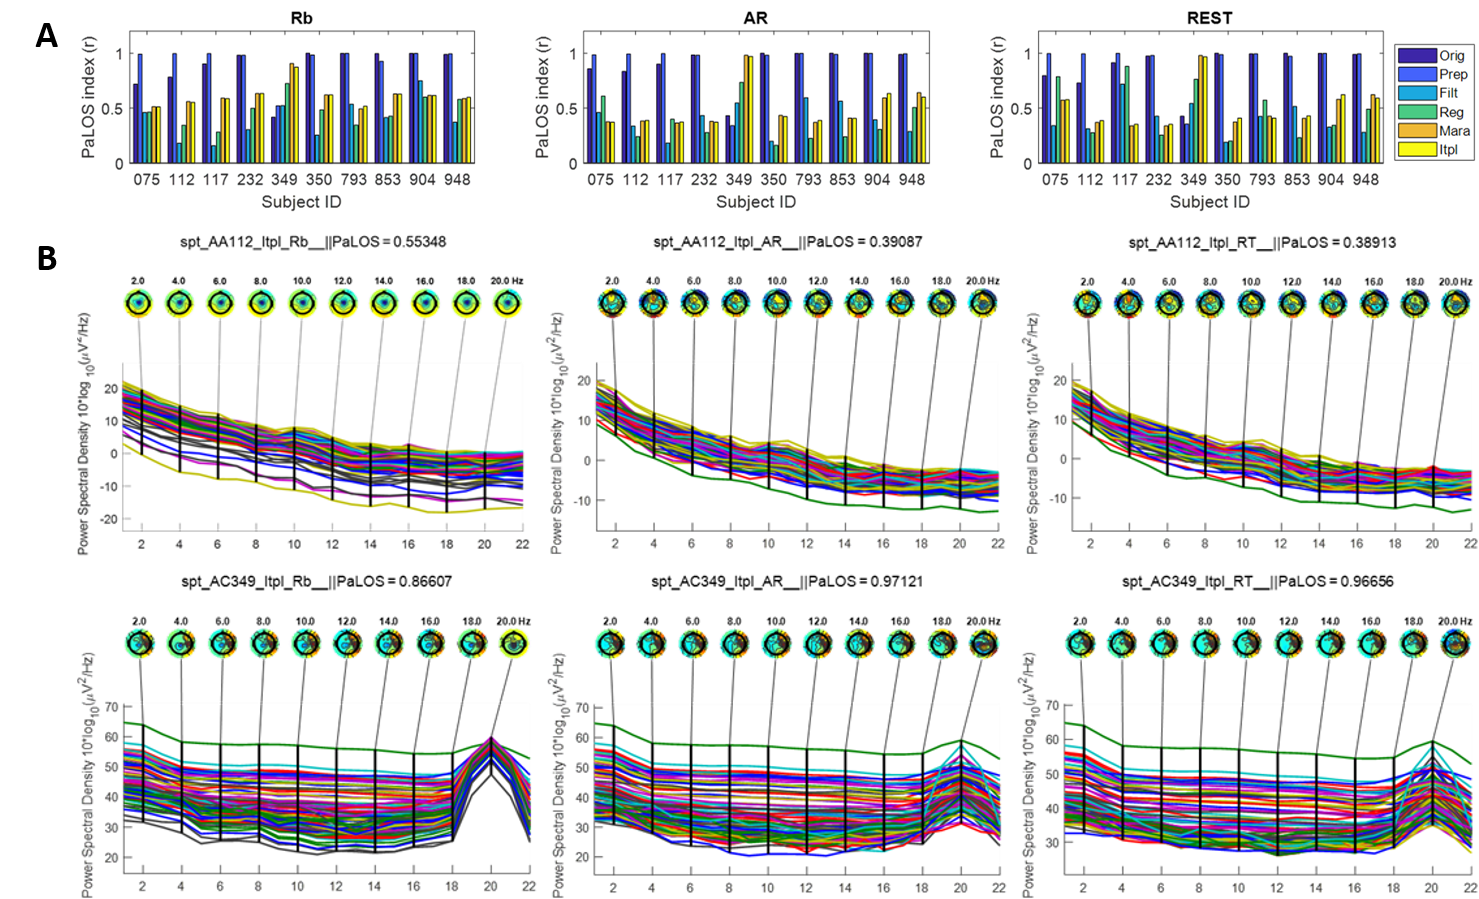
\includegraphics[width=15cm]{pic/palos/step.png}
	\caption{参考与预处理步骤分析。Rb:始于Cz的鲁棒平均参考,AR:传统平均参考,REST:零参考。 A. 谱同构指数随Automagic主要
	预处理步骤的变化趋势。 B. 第一行:谱异质的数据112,第二行:谱同构的数据349。}
	\label{step}
\end{figure}
为分析谱同构指数在不同预处理步骤和参考之间的差异,从CMI数据库中随机挑选10例数据,分别变换原始数据参考为Cz(在Automagic中重参考为鲁棒平均参考,Rb)、AR和REST再进行Automagic软件分步预处理。图\ref{step}A中表示三种参考情况下10例数据的谱同构指数随Automagic中原始数据(Orig)、坏道挑选(Prep)、滤波(Filt)、眼电回归(Reg)、伪差成分去除(MARA)和坏道插值(Itpl)步骤的变化。对Itpl步骤后的10例数据,Automagic软件基于脑电时域信息如幅度、方差、坏道比例等质量控制准则,不同参考下的质量控制结果一致,其中被试349、904质量为差,被试117、948质量为一般,其他数据为良好。不同参考下的10例数据总体上都表明应用坏道挑选(Prep)、眼电回归(Reg)和伪差成分去除(MARA)步骤会使谱同构指数上升,相比,滤波(Filt)步骤会使谱同构指数下降。质量为差的349、904数据的谱同构指数在Automagic分步处理中表现出与其它质量一般或良好的数据谱同构指数不同的分步变化趋势且Itpl步骤后的谱同构指数相对其它数据偏高。Prep步骤中去除坏道、Reg步骤中去除眼电、MARA步骤去除更多的伪差成分,特别是MARA步骤的独立成分分析去除的不同伪差成分和眼电、坏道统计学上接近相互独立代表原始数据中的异质性,应用这些步骤都使得脑电数据丢失异质信息从而谱同构指数升高。滤波(Filt)后谱同构指数下降主要是由于带通滤波去除了频率较低(<1Hz)的信息,而低频信息在谱曲线中对应较大的能量在原始数据中具有较大的幅度,因此去除低频信息丢失数据的同构信息,虽然丢失的高频信息代表数据的异质性,但因为高频对应幅度较低、谱曲线中能量很小,二者的抵消结果依然使数据丢失更多同构信息使谱同构指数下降。谱同构指数在噪声较强的数据预处理后下降但在预处理分步骤中可能出现上升再下降的趋势。数据的伪差程度不同,分步骤计算的谱同构指数的上升下降趋势就不一致。因为脑电的质量控制缺乏真正的基标准,还需要结合电生理专家的去伪差辅助分析,分析更多数据集找到不同伪差程度数据在预处理步骤中谱同构指数的变化趋势,甚至借助高性能计算平台进行大样本分析有望找到谱同构准则的阈值范围,实现对数据预处理质量的更加精准的控制。

图\ref{step}B中上下两行分别是一例好的数据112和一例差的数据349在不同参考下的多通道谱曲线和谱地形图分布。没有谱同构问题的112在三种参考下的谱同构指数为0.38-0.56,而具有谱同构问题的349在三种参考下谱同构指数为0.86-0.97,说明谱同构指数能表征实际是否存在谱同构的问题。不同参考间比较,对于112,AR和REST比Rb具有更符合谱异质情况的同构指数(0.39<0.55),对于349,AR和REST比Rb具有更符合谱同构情况的同构指数(0.97>0.86),但REST比AR对谱异质的112具有更小的同构指数,AR比REST对谱同构的349具有更大的同构指数。由此可见总体上REST和AR比Rb提供了更符合实际的谱同构指数证据,但REST和AR的差异并不明显。尽管不同参考不会影响自动化分析软件根据时域信息对数据的质量分类,但谱的同构异质性研究表明AR和REST比Rb更好。本章谱同构准则计算方法公开在https://github.com/ShiangHu/PaLOS-index.git中。

\section{本章小结}
本章发现预处理后脑电数据可能存在谱同构问题,基于共同主成分分析提出能表征脑电谱同构异质程度的PaLOS指数。结合自动化伪差去除和专家视觉挑选两种方法,在不同数据库中验证发现这种谱同构指数能有效表征多通道脑电时间序列预处理程度。谱同构准则有望作为大样本数据预处理后的一种初筛准则,避免因为应用强力预处理算法丢失掉与脑活动有关的信息而出现谱同构问题。